\section{Convolutional Neural Networks}
\label{convolutional_neural_networks}

Neuronale Netze \bzw{} Deep-Learning gehören zu den derzeit besten und beliebtesten Lösungen zu Problemen der Bild- oder Spracherkennung~\cite{Nielsen}.
Dabei lernt \bzw{} approximiert das Netz durch eine Anpassung ihrer Parameter über einer Menge an Trainingsbeispielen eine stetige Funktion, sodass die Trainingsbeispiele auf ihre gewünschte Ausgabe abbilden und auch für unbekannte Eingaben zuverlässige Vorhersagen getroffen werden können.
Neuronale Netze sind daher größtenteils in dem Bereich des \emph{überwachten maschinellen Lernens} anzuordnen.
Ein Netz, welches lediglich die Trainingsmenge lernt und dessen Parameter unbekannte Eingaben nicht generalisieren können, wird als ein \emph{überangepasstes} (\engl{} \emph{overfitted}) Netz bezeichnet~\cite{Nielsen}.

Ein \emph{neuronales Netz} besteht aus einer beliebigen Anzahl miteinander verbundener \emph{Neuronen}.
Neuronen sind üblicherweise mit anderen Neuronen in sequentiellen \emph{Schichten} \bzw{} \emph{Ebenen} angeordnet.
Die erste Schicht eines neuronalen Netzes wird als \emph{Eingabe}- und die letzte Schicht als  \emph{Ausgabeschicht} bezeichnet.
Schichten zwischen Ein- und Ausgabe heißen \emph{versteckt} (\engl{} \emph{hidden}).
Als \emph{Deep-Learning} wird ein Netz mit mindestens zwei versteckten Schichten verstanden.
Die einfachste Form eines neuronalen Netzes ist das \emph{Feedforward}-Netz, bei der jedes Neuron einer Schicht mit allen Neuronen der darauffolgenden Schicht verbunden ist.
Die Schichten eines Feedforward-Netzes werden deshalb auch als \emph{vollverbunden} (\engl{} \emph{fully-connected}) betitelt.
Abbildung~\ref{fig:feedforward} zeigt ein Beispiel eines solchen Netzes mit drei Schichten.
\begin{figure}[t]
\centering
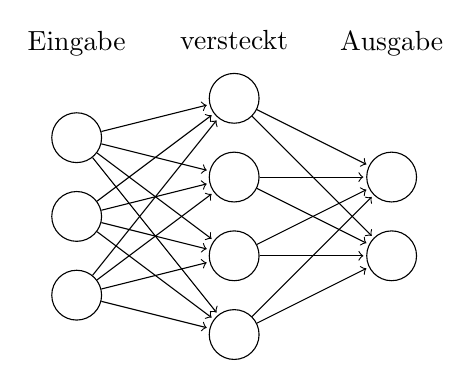
\begin{tikzpicture}
  \tikzstyle{node}=[circle,draw, minimum width=18pt, inner sep=0pt, fill=white]
  \tikzstyle{edge}=[->, shorten >= 1pt]

  \node[rectangle, inner sep=0pt] at (-2, 2.2) {Eingabe};
  \node[rectangle, inner sep=1pt] at (0,  2.24) {versteckt};
  \node[rectangle, inner sep=0pt] at (2,  2.2) {Ausgabe};

  \node[node] (a1) at (-2, -1) {};
  \node[node] (a2) at (-2, 0)  {};
  \node[node] (a3) at (-2, 1)  {};

  \node[node] (b1) at (0, -1.5) {};
  \node[node] (b2) at (0, -0.5) {};
  \node[node] (b3) at (0, 0.5)  {};
  \node[node] (b4) at (0, 1.5)  {};

  \node[node] (c1) at (2, -0.5) {};
  \node[node] (c2) at (2, 0.5)  {};

  \path[edge] (a1) edge (b1);
  \path[edge] (a1) edge (b2);
  \path[edge] (a1) edge (b3);
  \path[edge] (a1) edge (b4);
  \path[edge] (a2) edge (b1);
  \path[edge] (a2) edge (b2);
  \path[edge] (a2) edge (b3);
  \path[edge] (a2) edge (b4);
  \path[edge] (a3) edge (b1);
  \path[edge] (a3) edge (b2);
  \path[edge] (a3) edge (b3);
  \path[edge] (a3) edge (b4);
  \path[edge] (b1) edge (c1);
  \path[edge] (b1) edge (c2);
  \path[edge] (b2) edge (c1);
  \path[edge] (b2) edge (c2);
  \path[edge] (b3) edge (c1);
  \path[edge] (b3) edge (c2);
  \path[edge] (b4) edge (c1);
  \path[edge] (b4) edge (c2);
\end{tikzpicture}
\caption[Feedforward-Netz]{Beispiel eines Feedforward-Netzes mit drei vollverbundenen Schichten von einer Eingabe mit drei Neuronen zu einer Ausgabe mit zwei Neuronen und einer dazwischenliegenden versteckten Schicht.}
\label{fig:feedforward}
\end{figure}

Andere Netzvarianten erlauben \zB{} Schleifen, Rückwärtskanten oder das Überspringen einer Schicht~\cite{Nielsen}.

Ein Neuron besitzt genau einen reellen Wert, der sich aus den Neuronen der vorherigen Schicht erschließt.
Die $t$-te Neuronenschicht lässt sich folglich als ein Vektor $\ve{x}^{\left(t\right)} \in \gls{R}^{N^{\left(t\right)}}$ auffassen, wobei $N^{\left(t\right)} \in \gls{N}$ die Anzahl der Neuronen in der $t$-ten Schicht beschreibt.
Zu jeder Kante existiert zusätzlich ein Gewicht, welches den Anteil des Neurons zu dessen verbundenen Neuron angibt.
Damit lassen sich die Neuronenwerte der $\left(t+1\right)$-ten Schicht über
\begin{equation*}
  \ve{x}^{\left(t+1\right)} \coloneqq \gls{W}^{\left(t+1\right)}\ve{x}^{\left(t\right)}
\end{equation*}
definieren, wobei $\gls{W}^{\left(t+1\right)} \in \gls{R}^{N^{\left(t+1\right)} \times N^{\left(t\right)}}$ eine \emph{Gewichtsmatrix} der Kanten beschreibt, sodass $\gls{W}^{\left(t+1\right)}_{ji} \in \gls{R}$ das Gewicht der Kante des $i$-ten Neurons in der $t$-ten Schicht zu dem $j$-ten Neuron der $\left(t+1\right)$-ten Schicht angibt.
Zusätzlich zu den Gewichten existert zu jedem Neuron in der $t$-ten Schicht außer der Eingabeschicht ein \emph{Bias} $\gls{b}^{\left(t\right)} \in \gls{R}^{N^{\left(t\right)}}$.
Mit einer elementweisen Anwendung einer nicht-linearen \emph{Aktivierungsfunktion} $\gls{act} \colon \gls{R} \to \gls{R}$ ergibt sich damit die finale Version der Neuronenwerte der $\left(t+1\right)$-ten Schicht als
\begin{equation*}
  \ve{x}^{\left(t+1\right)} \coloneqq \gls{act} \left(\gls{W}^{\left(t+1\right)}\ve{x}^{\left(t\right)} + \gls{b}^{\left(t+1\right)} \right).
\end{equation*}
Als Aktivierungsfunktion kommt dabei \bspw{} die nicht-lineare \emph{Sigmoidfunktion} $\mathrm{sig}\left(z\right) \coloneqq 1 / \left(1 + \exp\left(-z\right)\right)$ oder die \emph{Rectified Linear Unit (ReLU)}-Funktion $\gls{relu}\left(z\right) \coloneqq \max \left(z, 0\right)$ zum Einsatz~\cite{Nielsen}.
Die Menge der Gewichte $\mathcal{W} \coloneqq {\left\{\gls{W}^{\left(t\right)}\right\}}_{t=2}^T$ sowie die Menge der Biaswerte $\mathcal{B} \coloneqq {\left\{\gls{b}^{\left(t\right)}\right\}}_{t=2}^T$ für $T \in \gls{N}$ viele Schichten werden die \emph{Parameter} des Netzes genannt, über dessen Anpassung das Netz trainiert wird.
Diese Werte werden dabei sequentiell über einer kleinen Eingabemenge $\mathcal{X}$ mit den Eingaben $\ve{x} \in \mathcal{X}$ so angepasst, dass eine stetige \emph{Kostenfunktion} minimiert wird.
Die Größe der Menge $\mathcal{X}$ wird dabei als \emph{Batch-Size} betitelt~\cite{Nielsen}.
Ein Beispiel einer Kostenfunktion ist die \emph{quadratische Kostenfunktion}, die über
\begin{equation}
  C\left(\mathcal{X}, \mathcal{W}, \mathcal{B}\right) \coloneqq \frac{1}{2\left|\mathcal{X}\right|} \sum_{\ve{x} \in \mathcal{X}} {\left\| \ve{y} - \ve{y}^{\prime} \right\|}_2^2
  \label{eq:quadratische_kostenfunktion}
\end{equation}
definiert ist, wobei \ve{y} die Ausgabe des Netzes und $\ve{y}^{\prime}$ die erwartete Ausgabe \bzgl{} \ve{x} beschreibt~\cite{Nielsen}.
Die implizit durch das Netz gegeben Werte $\mathcal{W}$ und $\mathcal{B}$ werden dabei oft weggelassen, sodass wir lediglich $C\left(\mathcal{X}\right)$ schreiben.





% Epoche
% Learning-Rate
% Loss-Function

% Receptive-Field
% Merkmalskarten oder Featuremap
% Backpropagation quelle
% Stride, Filtergröße
% Stride Slice Pooling
% genereller Faltungsoperator?
\gls{conv2d}
\gls{CNN}

% What we'd like is an algorithm which lets us find weights and biases so that the output from the network approximates y(x)y(x) for all training inputs xx. To quantify how well we're achieving this goal we define a cost function*

% Üblicherweise wird \gls{learning} so gewählt, dass nicht zu langsam gelernt wird, aber dennoch eine gute Approximation erreicht wird.
